
\documentclass[12pt]{article}

\usepackage{bbm}
\usepackage{float}
\usepackage{caption, subcaption}
\usepackage[T1]{fontenc}
\usepackage[backend=bibtex, maxbibnames=99, sorting=none]{biblatex}
\addbibresource{sample.bib}
\usepackage{url}
\usepackage[utf8]{inputenc}
\usepackage{booktabs} % For prettier tables
\usepackage{siunitx} % For aligning numbers at the decimal point
\usepackage{caption} % For captions
\usepackage{amsmath}
\usepackage{graphicx}
\usepackage{subcaption}
\usepackage{setspace}
\usepackage{graphicx}
\usepackage{subcaption}
\usepackage{amssymb}
\graphicspath{{Images/}}
\usepackage{parskip}
\usepackage{multirow}
\usepackage{enumitem}
\usepackage{amssymb}
\usepackage{framed}
\usepackage{fancyhdr}
\usepackage{vmargin}
\usepackage{subcaption} %usamos subcaption mejor que subfig (más moderno)
\usepackage{eurosym}
\usepackage[table,xcdraw]{xcolor} % add color to your tables
\usepackage[bottom]{footmisc} %footnotes
\definecolor{blau}{RGB}{210,235,255}
\definecolor{blau2}{RGB}{120,170,225}
\setmarginsrb{2.5 cm}{2 cm}{2 cm}{2.5 cm}{1 cm}{0.5 cm}{1 cm}{1 cm}

\usepackage{multirow}

\usepackage{chngcntr}

\usepackage[framed, numbered]{matlab-prettifier}
 
\counterwithin{figure}{section}
\counterwithin{table}{section}
\numberwithin{equation}{section}

\usepackage{titlesec}
\usepackage{hyperref}
\usepackage{listings}
\usepackage{multicol}
\setlength{\columnsep}{1cm}

\titleclass{\subsubsubsection}{straight}[\subsection]

\newcounter{subsubsubsection}[subsubsection]
\renewcommand\thesubsubsubsection{\thesubsubsection.\arabic{subsubsubsection}}
\renewcommand\theparagraph{\thesubsubsubsection.\arabic{paragraph}} % optional; useful if paragraphs are to be numbered

\titleformat{\subsubsubsection}
  {\normalfont\normalsize\bfseries}{\thesubsubsubsection}{1em}{}
\titlespacing*{\subsubsubsection}
{0pt}{3.25ex plus 1ex minus .2ex}{1.5ex plus .2ex}

\makeatletter
\renewcommand\paragraph{\@startsection{paragraph}{5}{\z@}%
  {3.25ex \@plus1ex \@minus.2ex}%
  {-1em}%
  {\normalfont\normalsize\bfseries}}
\renewcommand\subparagraph{\@startsection{subparagraph}{6}{\parindent}%
  {3.25ex \@plus1ex \@minus .2ex}%
  {-1em}%
  {\normalfont\normalsize\bfseries}}
\def\toclevel@subsubsubsection{4}
\def\toclevel@paragraph{5}
\def\toclevel@paragraph{6}
\def\l@subsubsubsection{\@dottedtocline{4}{7em}{4em}}
\def\l@paragraph{\@dottedtocline{5}{10em}{5em}}
\def\l@subparagraph{\@dottedtocline{6}{14em}{6em}}
\makeatother

\usepackage[table,xcdraw]{xcolor}

\setcounter{secnumdepth}{4}
\setcounter{tocdepth}{4}


\usepackage{pdflscape} %Per poder posar la pàgina en horizontal
\usepackage{multicol} %Escriure en columnes 
 
	% Author
\date{\today}							% Date

\makeatletter
\let\thetitle\@title
\let\theauthor\@author
\let\thedate\@date
\makeatother

\pagestyle{fancy}
\fancyhf{}
\lhead{21D009 Networks: Concepts and Algorithms}
\rhead{Movie recommendations using networks}
\cfoot{\thepage}

\begin{document}

\begin{titlepage}
	\centering
    
\includegraphics[scale = 0.7]{bse_logo.png}\\[1.2 cm]	% University Logo
    \textsc{\LARGE Barcelona School of Economics}\\[2.0 cm]	% University Name
	\textsc{\Large Data Science Methodology Program}\\[0.5 cm]				% Course Code
	\textsc{\large 21D009 Networks: Concepts and Algorithms }\\[0.5 cm]				% Course Name
	\rule{\linewidth}{0.2 mm} \\[0.4 cm]
	{ \huge \bfseries Movie recommendations using networks }\\
	\rule{ \linewidth}{0.2 mm} \\[1.5 cm]
	
\begin{center}
    
{ \emph{Authors: }\\
    \textsc{Codd}, Jonny \\
    \textsc{Chen}, Joshua \\
    \textsc{Gallegos}, Rafael \\
    \textsc{Pérez}, Carlos \\ } 

\vspace{0.7cm}


    \textit{Professors:}\\  \textsc{Milán}, Pau \\
    	\textsc{Komander}, Björn
        \\ \vspace{0.5cm}


\vspace{1.7cm}


{\large December $20^{th}$, 2023} \\[2 cm]

 \end{center}
	\vfill
	
\end{titlepage}
	
\tableofcontents
\vspace{1cm}
\listoffigures
\listoftables
\pagebreak

\newpage

\section{Introduction}

Popular recommendation techniques in Machine Learning often apply many network and network-adjacent concepts to create personalized recommendations. The matrix of user-to-item scores can be thought of as the adjacency matrix of a bipartite network - with the users representing one set of nodes and the items representing the other. The edges are represented either by binary or scalar relationships between users and items, implying unweighted or weighted graphs respectively.

Our project is two-fold. Using the concepts learned in this course, we will first analyze one of these networks to identify trends and patterns and extract information. We will then study and build recommendation systems and propose/implement new strategies and techniques derived from the first part to improve methodologies.

\section{Literature Review}

\section{Dataset}

MovieLens is popular movie recommender system dataset developed by GroupLens, a computer science research lab at the University of Minnesota. The goal of this challenge is to recommend movies to its users based on their movie ratings. Group Lens offers datasets of different sizes and their datasets are widely used in research and teaching contexts.

The selected dataset consists mainly on two files: movies.csv and ratings.csv. Movies dataset has 9,742 unique films and a column indicating the genres of the film. All possible genres are: 'Romance', 'Musical', 'Children', 'Documentary', 'Sci-Fi', 'Film-Noir', '(no genres listed)', 'Crime', 'Mystery', 'Drama', 'Western', 'Fantasy', 'Animation', 'Thriller', 'War', 'Action', 'Adventure', 'IMAX', 'Comedy', 'Horror'. The number of movies per genre is represented in Figure \ref{fig:count_genre}.

Ratings dataset consists of 100,836 ratings with 610 unique users that rated 9,724 movies. As it can be observed in Figure \ref{fig:count_rating}, the ratings from users are right-skewed, which suggests that users tend to enter their rating on movies that they probably have liked. Ratings from users have been registered from 1996-03-29 until 2018-09-24. The most popular movies among users have been: Shawshank Redemption, The (1994), Godfather, The (1972), Fight Club (1999), Godfather: Part II, The (1974) and Goodfellas (1990).

\begin{figure}[h!]
    \begin{minipage}[b]{0.49\linewidth}
         \centering
  	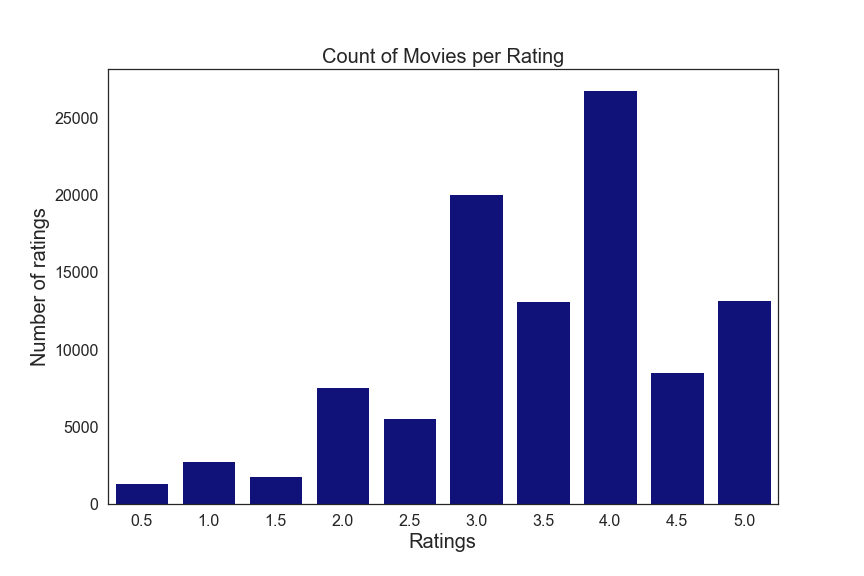
\includegraphics[width=0.99\textwidth]{count_rating.png}
  	\caption{Count of Movies per Rating}
  	\label{fig:count_ranking}
    \end{minipage}
    \hspace{0.01cm}
    \begin{minipage}[b]{0.49\linewidth}
        \centering
  	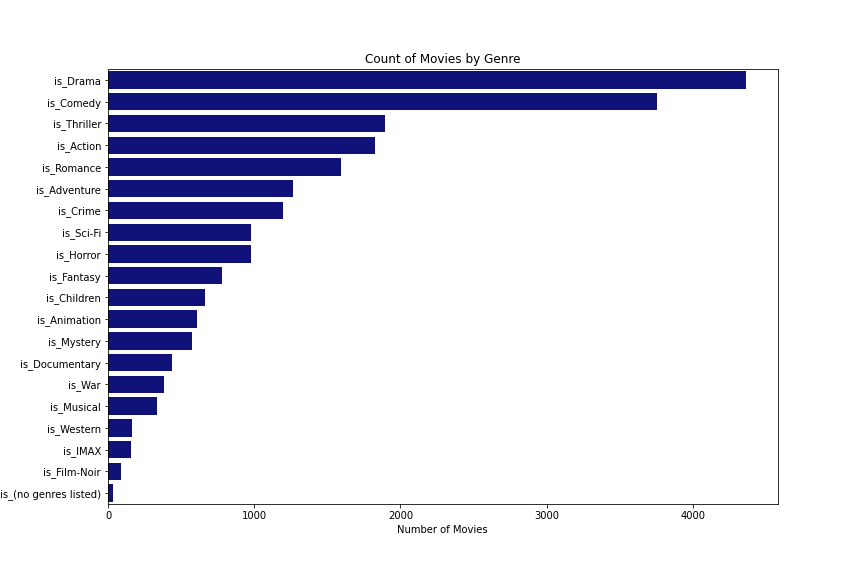
\includegraphics[width=0.99\textwidth]{count_genre.png}
  	\caption{Count of Movies per Genre}
  	\label{fig:count_genre}
    \end{minipage}
\end{figure}

The median user has rated 70 films, whereas the user with the lowest number of watched films was 20 movies and the user with the highest number of rated films is 2698.

\begin{figure}[h!]
    \begin{minipage}[b]{0.49\linewidth}
         \centering
  	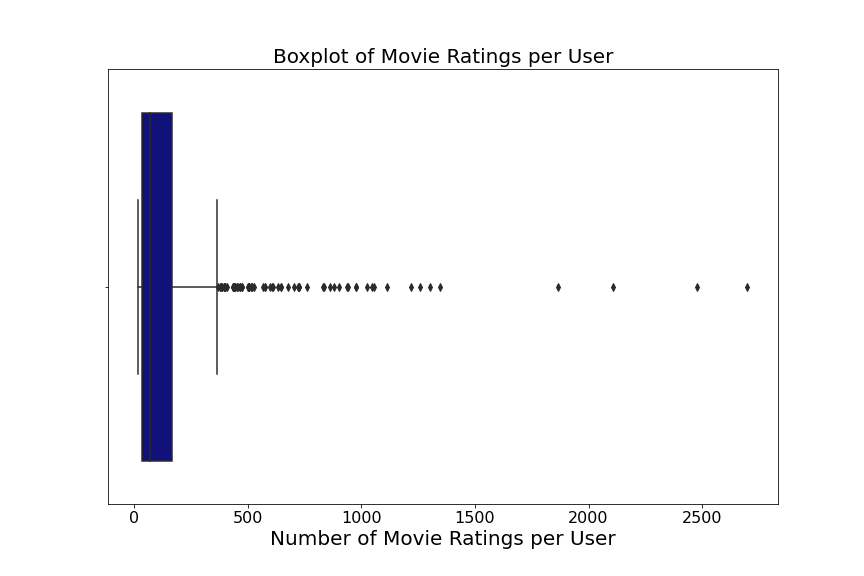
\includegraphics[width=0.99\textwidth]{count_user.png}
  	\caption{Count of Movies per User}
  	\label{fig:count_user}
    \end{minipage}
    \hspace{0.01cm}
    \begin{minipage}[b]{0.49\linewidth}
        \centering
  	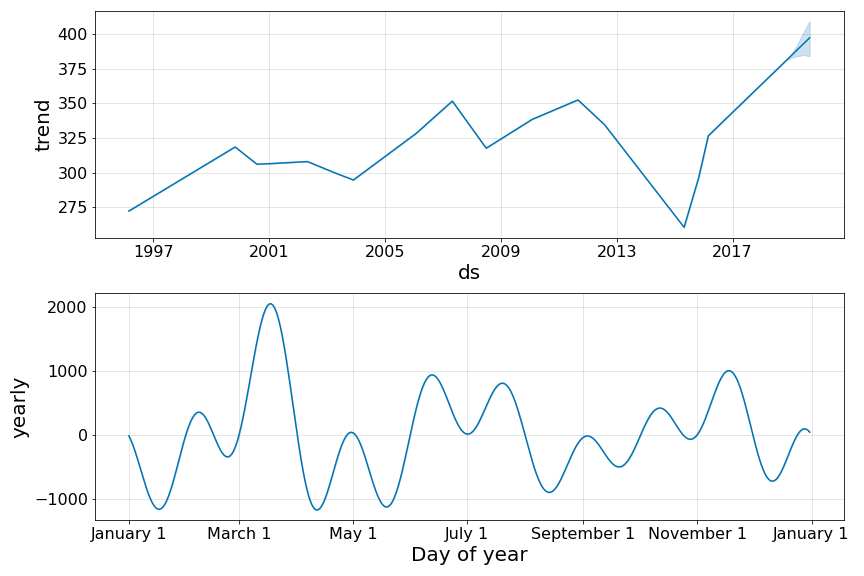
\includegraphics[width=0.99\textwidth]{prophet.png}
  	\caption{Time Series Analysis of Ratings with Prophet}
  	\label{fig:ranking_ts}
    \end{minipage}
\end{figure}

\section{Network analysis}

With the MovieLens dataset, we created 4 different networks.  The first, the user-movie network, is the aforementioned user-item network that will serve as the foundation for both the other networks and the recommendation systems that we build. From this network, we also
constructed a user-to-user network - a symmetric unipartite network capturing the similarity between users. Similarly, we did this for the movies as well. Finally, we created another bipartite network that, instead of capturing relationships between users and specific movies, it describes the "fan score" between a user and a genre of movie.

\subsection{User and movie bipartite network}

To create the user/movie bipartite network, we used the Networkx package in Python. We selected the unique User Ids as one set of nodes and the movie titles as another. Edges were then added if a user has seen a movie. Note that this is a undirected, unweighted graph. Ratings are not considered here.

Despite an incredibly sparse matrix, understandably with close to 10,000 movies - this results in a connected graph - meaning there is only one component.

\begin{figure}[h!]
\centering
    \begin{minipage}[b]{0.49\linewidth}
         \centering
  	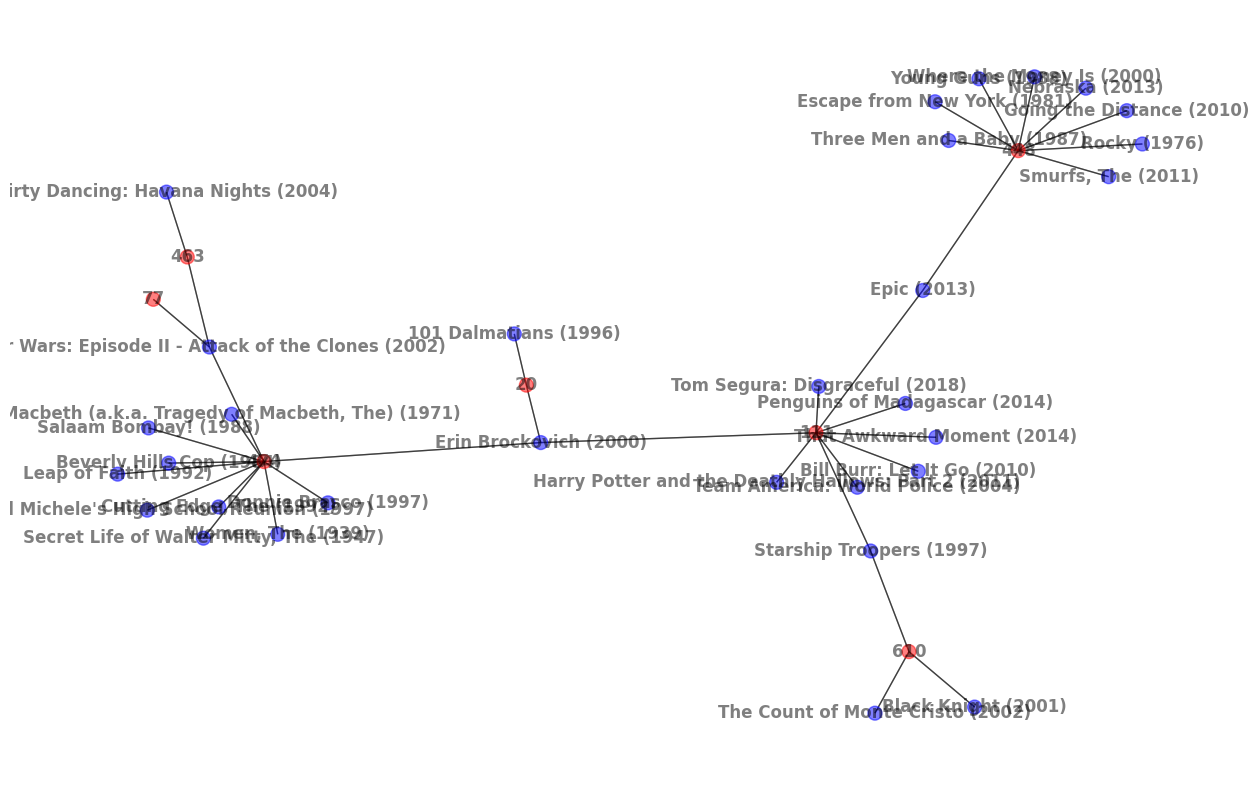
\includegraphics[width=0.99\textwidth]{sample_graph.png}
  	\caption{Subset of User to Movie Network}
  	\label{fig:count_ranking 2} 
    \end{minipage}
    \hspace{0.01cm}
    \begin{minipage}[b]{0.49\linewidth}
        \centering
  	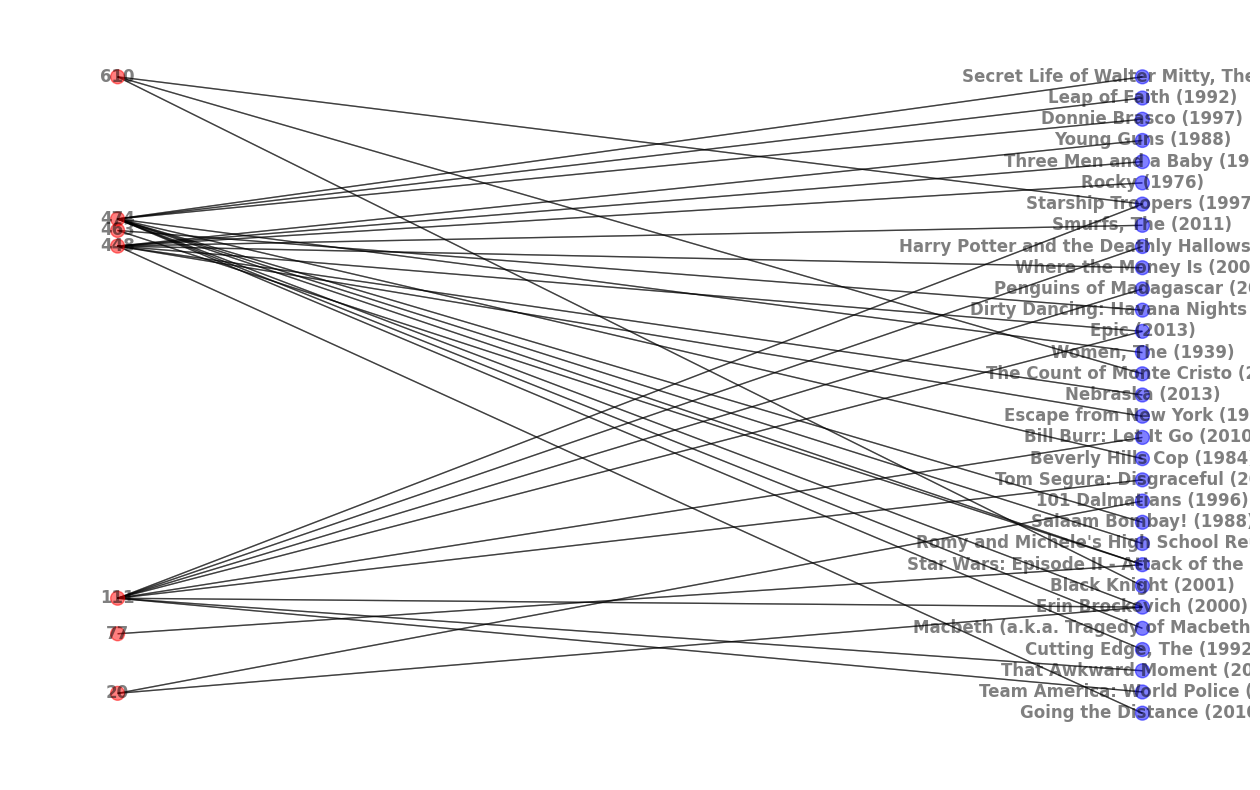
\includegraphics[width=0.99\textwidth]{bipartite.png}
  	\caption{BipartiteLayout}
  	\label{fig:ranking_ts 2}
    \end{minipage}
\end{figure}


To better understand that users and movies, we calculated the centrality for each of them:
With this graph - the degree centrality for users and movies are aligned with how many reviews they have. The centrality score for users is much higher than that for movies as there are many more reviews per user than there are per movie. 

However, this may not be the best way to actually capture centrality as highly central movies and users might not just be how many direct nodes that they have. Therefore, we also calculated the betweenness and closeness centralities. Take, for example, The Avengers (2012). Regardless of how many reviews it may have, it will probably be an important bridge (betweeness) between the Marvel movies. It is relationships like these that we are hoping to capture. However, there seems to be very little difference in the rankings of these centrality metrics as the top scores keep generally the same order. A couple near the bottom were pushed down but there was no large shuffling.

\begin{figure}[h!]
\centering
\caption{Network Centrality Measures and Comparative Metrics for Movies}
    \begin{tabular}{|c|c|c|c|}
        \hline
        \textbf{User Id} & \textbf{Degree Centrality} & \textbf{Betweeness Centrality} & \textbf{Closeness Centrality} \\ 
        \hline
        599 & 4.067 & 0.141 (1) & 0.406 (2) \\
        414 & 4.429 & 0.131 (2) & 0.413 (1) \\
        474 & 3.460 & 0.120 (3) & 0.395 (3) \\
        448 & 3.061 & 0.110 (4) & 0.388 (4) \\
        274 & 2.210 & - & 0.373 (5) \\
        610 & 2.136 & 0.060 (5) & 0.372 (6) \\
        68  & 2.067 & - & 0.371 (7) \\
        380 & 2.000 & 0.034 (10) & 0.370 (8) \\
        606 & 1.829 & 0.050 (6) & 0.367 (9) \\
        288 & 1.731 & - & 0.365 (10) \\
        \hline
    \end{tabular}

   \vspace{0.2cm} % Adjust the vertical space between tables as needed
    
    \begin{tabular}{|p{6cm}|r|r|r|}
        \hline
        \textbf{Movie Title} & \multicolumn{1}{p{2.5cm}|}{\textbf{Degree Centrality}} & \multicolumn{1}{p{3cm}|}{\textbf{Betweeness Centrality}} & \multicolumn{1}{p{3cm}|}{\textbf{Closeness Centrality}} \\
        \hline
        Forrest Gump (1994) & 0.0339 & 0.0064 & 0.4824 \\
        Pulp Fiction (1994) & 0.0316 & 0.0050 & 0.4650 \\
        Matrix, The (1999) & 0.0286 & 0.0048 & 0.4694 \\
        The Silence of the Lambs (1991) & 0.0287 & 0.0046 & 0.4624 \\
        Shawshank Redemption (1994) & 0.0326 & 0.0042 & - \\
        Star Wars: Episode IV (1977) & 0.0258 & 0.0041 & 0.4613 \\
        Jurassic Park (1993) & 0.0245 & - & - \\
        Braveheart (1995) & 0.0244 & - & - \\
        Terminator 2 (1991) & 0.0231 & - & - \\
        Schindler's List (1993) & 0.0226 & - & - \\
        \hline
    \end{tabular}
\end{figure}

It is important to note already that the most highly centralized movies are all produced before 2000 (in fact, this extends far beyond just the top 10), despite most of the reviews coming after the 2020s. This is understandable as movies that have been around longer are more likely to have more reviews.

\subsection{User-to-user network}

To construct the user-to-user network, we calculated the similarity between all users as our edges.  We first pivoted the Ratings dataframe on the \textit{UserId}. Our resulting dataframe has the UserId as the index, the Movies as the columns, and any user ratings inside. This is exactly the adjacency matrix for the User to Movie network that we created in the previous section; however, just weighted edges based on ratings.

We used cosine similarity as our node embedding technique to map user vectors into Euclidean space. Cosine similarity is a common space because it ignores magnitude and focuses only on directions in space. For example, A harsh critic might rate an average movie a 2 but a more generous critic might consider average to be 3. This would not affect at all the cosine similarity (if we kept the ratings positive). A similarity measure such as Euclidean distance would fail here because the more movies you add can only possibly add distance. Therefore people are punished for actually having seen more of the same films.

Because this is an incredibly sparse matrix, in order to calculate similarity scores, we only used the films that people had shared reviews for. However, this could result in the case where two people are assigned similarities despite having very little in common. For example, if two people who have wildly different preferences watched one random movie and both gave it 4 stars, these two people would be assigned a perfect similarity when, clearly, this should not be the case. To mitigate this, we only kept similarity scores for people that have rated 10 or more movies in common.

We actually calculated two similarity scores. Because ratings are all positive, all vectors will only be in the positive space. Therefore, cosine similarities are limited to only positive values as any two vectors cannot exceed more than a right angle. We constructed a similarity matrix using this framework which will henceforth in the paper be referred to as simply the User Network.

However, we also constructed another network where we subtracted 2.5 from all ratings. This allows for negative cosine similarities but has two important implications. First, in the example above regarding the harsh vs the generous critic, this is no longer true as now, their vectors are directly opposite (-0.5 vs 0.5). This model will be less able to adjust for user biases within their personal ratings. However, a large benefit of this approach is that it also captures \textit{dissimilarity} as well. For example, if two users have seen the same movie but have rated it 0.5 and 5.0, while these ratings are clearly diametrically opposed, this still add similarity towards their score. Now, when we subtract 2.5, essentially set 2.5 as the "neutral" threshold. Anything below is considered negative and anything above is considered positive. Users who share negative or positive scores will be rewarded with similarity and users who have disagreements will negative similarity. This network will henceforth be referred to as the Midrange-Adjusted User Network.

Again, these similarities can be conceived of as an adjacency matrix - this for a unipartite, weighted, bidirectional graph (i.e. the matrix is symmetric as the similarity from user a to user b is the same as user b to user a). From these graphs we made an unweighted graph by setting a threshold of 0.9 for the User Network and 0.5 for the Midrange-Adjusted User Network. These thresholds were chose as they both return similar numbers of edges (around 68,000). If the similarity score is greater than the threshold, an edge is created.

\begin{figure}[h!]
    \begin{minipage}[b]{01\linewidth}
         \centering
  	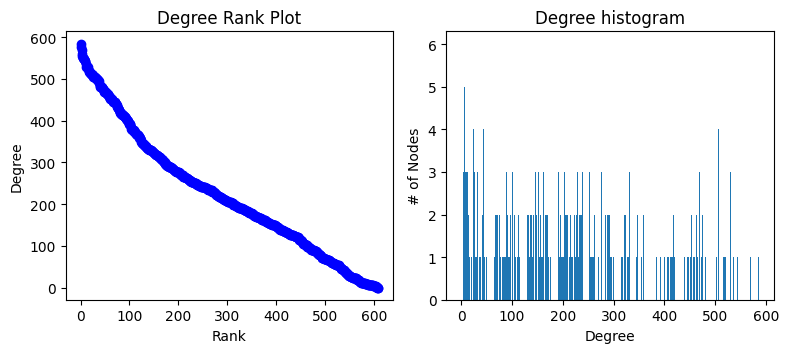
\includegraphics[width=0.9\textwidth]{UN_degreeinfo.png}
  	\caption{Degree Information for User Network}
  	\label{fig:UN_degreeinfo}
    \end{minipage}
\end{figure}

\subsection{Movie-to-Movie network}

\subsection{User-to-Genre network}

Many recommendation systems, including Random Walks and Collaborative Filtering which we will discuss later, only take into account user and item interactions. The content of the films is irrelevant and no relationship between the items is captured beyond what was described in the matrices above. Clearly, if we were able to capture these relationships, we could then build much stronger recommendations. One simple ubiquitous covariate is the genre of the film. It wouldn't feel quite right to sit down for family movie night and be recommended The Shining because you watched The Lion King last week - despite both movies probably having somewhat similar cosine similarity as both movies are generally well regarded. Item-to-item recommendations should consistently stay within the same category and, often, user-recommendations are filtered by said categories.

Therefore, we took a network approach to deepen our understanding between users and genres. Our goal is to quantitatively capture relationships between users and genres to provide better recommendations. In order to do this, we first classified out movies. The movie dataset contains a string of genres separated by a |. We split up the string and then filtered each movie into their respective genres. Movies with no listed genres were dropped. We then calculated the average rating per person as well as the average rating per genre per person. We also counted, the total number of reviews, as well as the total number of reviews per genre. 

For each genre, we then had to create a formula to determine whether or not someone was a fan of a genre. We settled on the following formula:

\[
\text{F}_{gi}= \text{tanh}\left(\frac{P_{gi} R_{gi}\ln(C_{gi})}{3}\right)
\]

$P_g$ is the percentage of user reviews within genre $g$. Naturally, if a larger percentage of a person's movies belong to a single genre, this should be rewarded. Similarly, $R_g$ represents the average review for a user within a genre. The higher the reviews, the greater the score. Finally, we wanted to factor in the number of films within the genre watched. While this should be somewhat accounted for in $P_g$, this may be helpful for identifying super fans or "influencers". This is reward logarithmically and we divide by 3 as a scaling constant.
This is then passed through tanh to give us fan scores between 0 and 1 (as this score can never be negative unless we adjust with midrange which then could capture a possible "hater score").

Then we arbitrarily chose 0.8 as the threshold. For users with over a 0.8, they were considered a fan. 

\begin{figure}[h!]
    \begin{minipage}[b]{0.49\linewidth}
         \centering
  	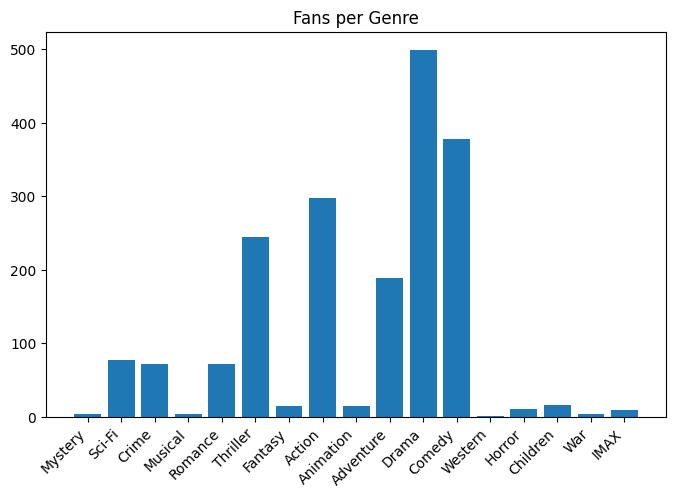
\includegraphics[width=0.99\textwidth]{fans_per_genre.png}
  	\label{fig:fanspergenre}
	 \caption{Fans per Genre}
    \end{minipage}
    \hspace{0.01 cm}
    \begin{minipage}[b]{0.49\linewidth}
         \centering
  	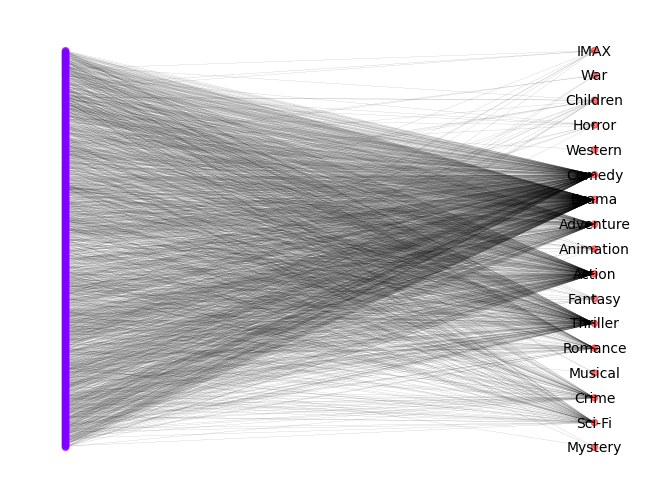
\includegraphics[width=0.99\textwidth]{genre_bipartite.png}
  	\caption{\\Users - Genre Bipartite Graph}
  	\label{fig:genre_bipartite}
    \end{minipage}
\end{figure}

Once again, we can create an unweight bipartite adjacency matrix from this with, the users as one set of nodes and the movies as the other (visualized in Figure 4.6).

Here, the degree represents how the number of genres for which that user is considered a fan. With the degree histogram, we see a strong fit of a binomial distribution with $n = 19$ (the number of genres) and $p = \frac{4.5}{19}$

\begin{figure}[h!]
    \begin{minipage}[b]{1\linewidth}
         \centering
  	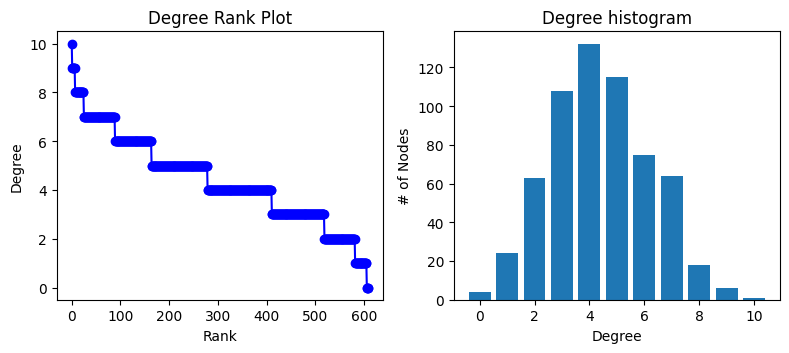
\includegraphics[width=0.99\textwidth]{genre_degree1.png}
  	\label{fig:fanspergenre}
	 \caption{User Degrees}
    \end{minipage}
    \vspace{0.1cm}
    \begin{minipage}[b]{1\linewidth}
         \centering
  	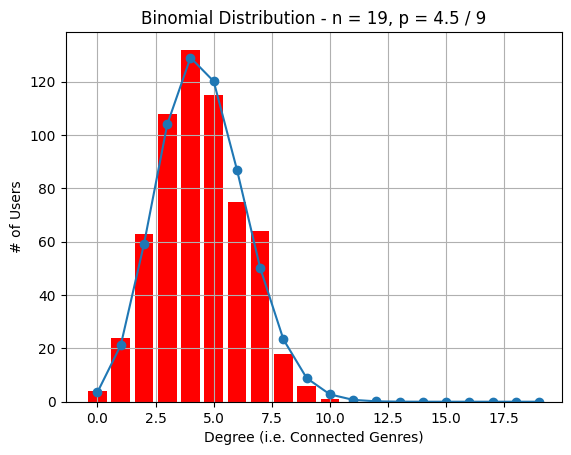
\includegraphics[width=0.5\textwidth]{binomialfit.png}
  	\label{fig:fanspergenre}
    \end{minipage}
\end{figure}

However, looking at Figure 4.5, we see an issue. It appears here that we are just measure how many movies there are per genre. Our formula, while it could be effective for large relatively balanced sets, fails in this context. Therefore, we will attempt to create a definition of "fan" that is more accounts for movie imbalances.

\[
F_{gi}^* = \left(\frac{R_{gi} - R_i}{R_g}\right)\mathbbm{1}{\{C_g > 10\}}
\]

This simplified version finds the difference between a user's score per genre with the average rating per genre and normalizes it by the average rating of that user. The threshold for being a fan here was set to 0.5. Here are the results:
\begin{figure}[h!]
\centering
    \begin{minipage}[b]{0.5\linewidth}
         \centering
  	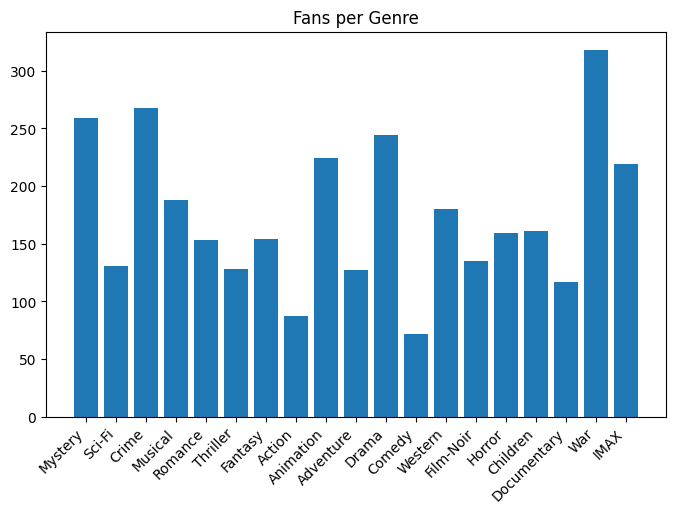
\includegraphics[width=0.99\textwidth]{fansgenre1.png}
  	\label{fig:fanspergenre}
	 \caption{New Fans per Genre}
    \end{minipage} 
\end{figure}

\begin{figure}[h!]
    \begin{minipage}[b]{0.5\linewidth}
         \centering
  	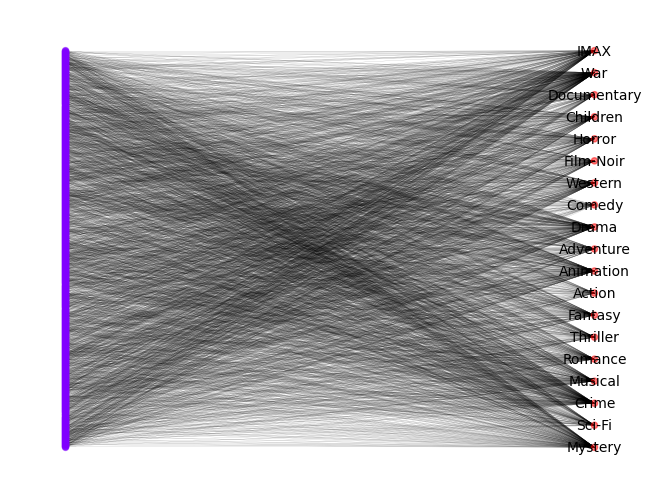
\includegraphics[width=0.99\textwidth]{newgenrebipartite.png}
  	\label{fig:fanspergenre}
	 \caption{New User-Genre Bipartite Graph}
    \end{minipage} 
    \hspace{0.1cm}
    \begin{minipage}[b]{0.5\linewidth}
         \centering
  	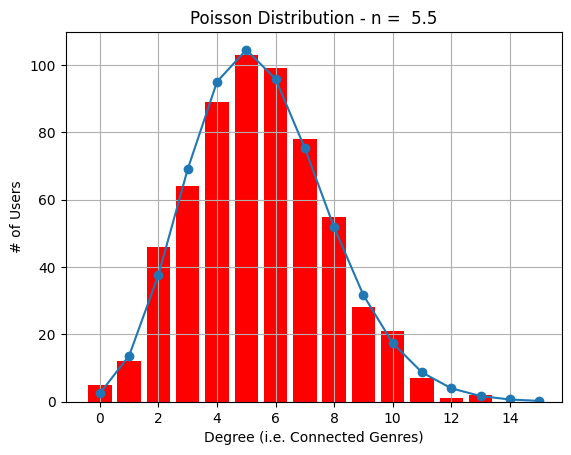
\includegraphics[width=0.99\textwidth]{poissondegree.png}
  	\label{fig:fanspergenre}
	 \caption{Poisson fit with $n = 5.5$}
    \end{minipage} 
\end{figure}

The distribution of fans across genres is now much more even and the degree distribution among fans aligns closely a Poisson with mean 5.5.

\section{Random Walk Models}

In this section, we explore recommendation systems that directly leverage the network structure of the data. In particular, we consider Probabilistic Spreading (ProbS) and Heat Spreading (HeatS) algorithms which are based off a random walk process which directly use a binary user-items bipartite network to provide a ranking to movies that they have not seen.

In this section, we explore recommendation systems that directly leverage the network structure of the data. Specifically, we focus on the Probabilistic Spreading (ProbS) and Heat Spreading (HeatS) algorithms, which employ a random walk process within a binary user-item bipartite network. 

For a given user \textit{i} , the ProbS algorithm initialises by giving a unit amount of resource to all items that they are connected to. The algorithm then employs a two-step random walk process to redistribute these resources, aiming to accentuate items preferred by users with similar tastes.

In the first step, each item's allocated resource is evenly distributed among users connected to it. This step effectively maps out the extent of shared interests between users based on the items they are associated with. Subsequently, the second step redistributes the resources accumulated by each user back to the items they are connected to, but now the distribution is equal among all such items. Through this reciprocal resource exchange, the algorithm iteratively refines the weight or importance of each item based on the density and depth of shared user preferences. Finally, the scores of items already connected with user \textit{i} are set to zero so as to not recommend items already connected with the user. A graphical representation of this process is shown in Figure \ref{subfig:prob_s}.

HeatS works in a very similar way to ProbS except a nodes score in the first and second steps are calculate as a simple average of the nodes it is connected to. A  graphical representation of this process is shown in Figure \ref{subfig:heat_s}.

\begin{figure}[!ht]
\centering
\begin{subfigure}[b]{0.45\textwidth}
    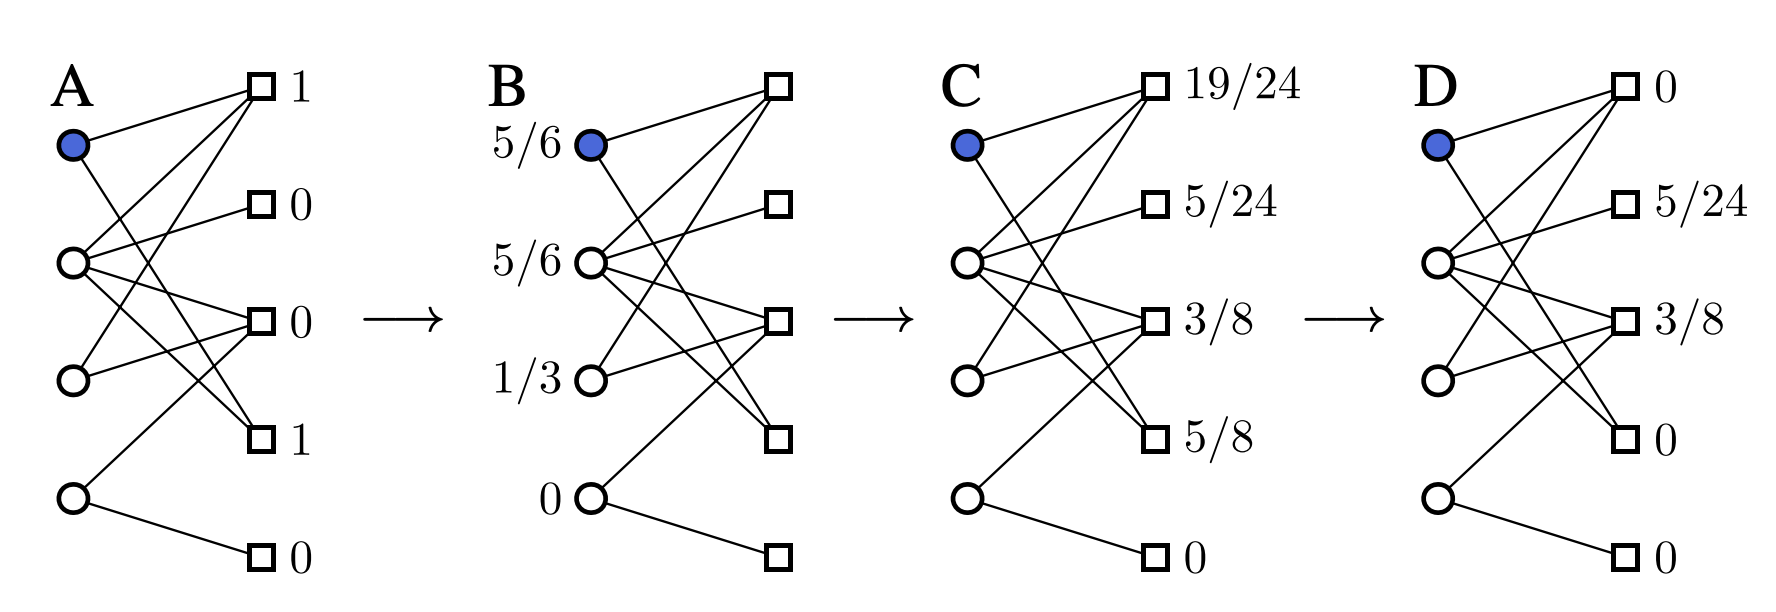
\includegraphics[width=\textwidth]{Prob S algorithm}
    \caption{ProbS Algorithm}
    \label{subfig:prob_s}
\end{subfigure}
\hfill % This adds space between the two subfigures
\begin{subfigure}[b]{0.45\textwidth}
    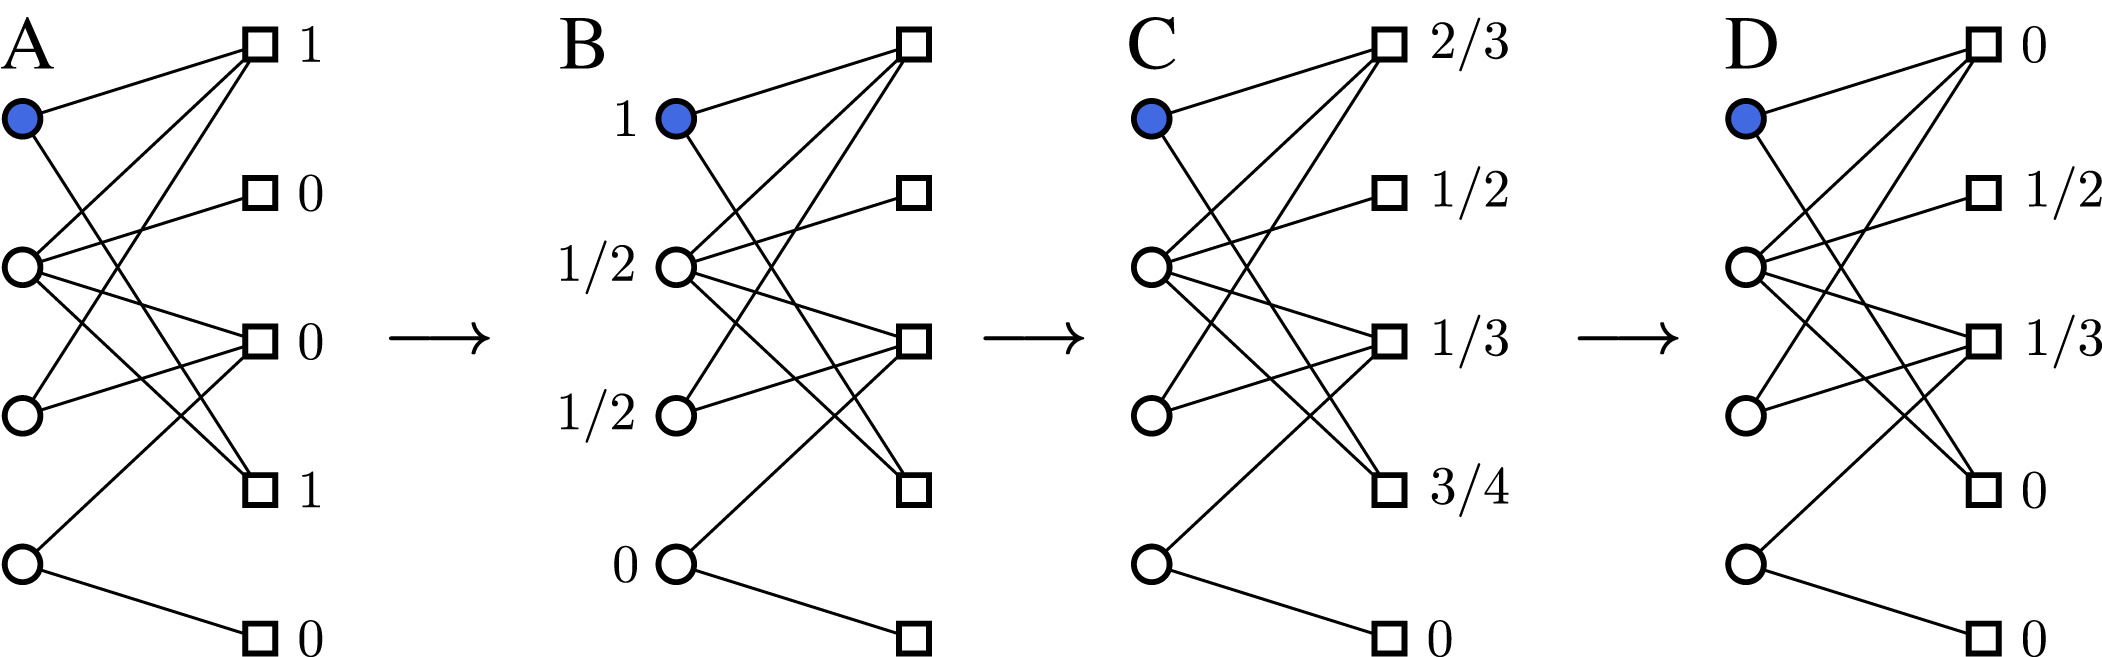
\includegraphics[width=\textwidth]{Heat S.jpg}
    \caption{HeatS Algorithm}
    \label{subfig:heat_s}
\end{subfigure}
\caption{Illustrations of the Probabilistic Spreading (ProbS) and Heat Spreading (HeatS) algorithms. In both diagrams, circles and squares represent users and items, respectively. The color-marked circle signifies the target user for whom the recommendations are being computed. Figures adapted from \cite{YU2016192}.}
\label{fig:algorithms}
\end{figure}

Although the distinction between the two algorithms is subtle, there is a stark difference between the recommendations they produce. The ProbS method exhibits a stronger preference for popular items as the process is cumulative; therefore, an item enhances its likelihood of achieving a high score by accumulating numerous links. In contrast, the HeatS approach tends to favour less popular items. This preference is due to the averaging nature of the HeatS algorithm, where an item can increase its potential for a high score by having a limited number of links to users who possess a significant amount of resource value. This distinction between the two methods highlights their unique approaches to leveraging network dynamics, where ProbS capitalizes on the popularity and widespread connectivity of items, whereas HeatS leverages the principle of scarcity and targeted endorsements from highly resourced users.

As an extension of these algorithm, we also experiment with initialising weights proportional to the rating a user gave each movie. By doing so, we hope to provide prioritise movies that the user enjoyed more, potentially leading to more tailored recommendations. 


\subsection{Temporal Analysis}

To gain deeper insights into the long-term effects of these recommendation algorithms, we examine the evolving dynamics of the network with iterative applications of the algorithm. In each cycle, we posit that the user selects and watches the top-recommended movie, subsequently leading to an update of the binary bipartite network to reflect this new user-item interaction. The recommendation algorithm is then reapplied, taking into account the updated state of the network. This process is repeated, allowing us to observe how the network—and thus the recommendations—might evolve over time with continuous user engagement.

Figure \ref{fig:temporal prob S} shows the recommendation counts after 1,  10 and 100 iterations of the binary ProbS algorithm, and the effect this has on the degree of each user.  The recommendation counts clearly illustrates a power-law distribution, indicating a strong preference by the algorithm for particular items. As a result, certain movies become highly connected, reaching a saturation point where nearly all users have watched with them. This saturation compels the algorithm to diversify its recommendations, thereby incrementally expanding the range of movies suggested to users. 


\begin{figure}[!ht]
\centering

% First row with three figures
\begin{subfigure}[b]{0.32\textwidth}
    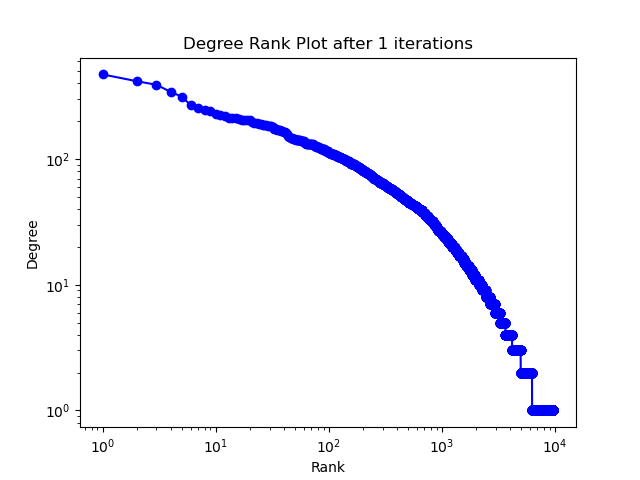
\includegraphics[width=\textwidth]{Prob S movie rank plot - 1 iterations.png}
\end{subfigure}
\hfill
\begin{subfigure}[b]{0.32\textwidth}
    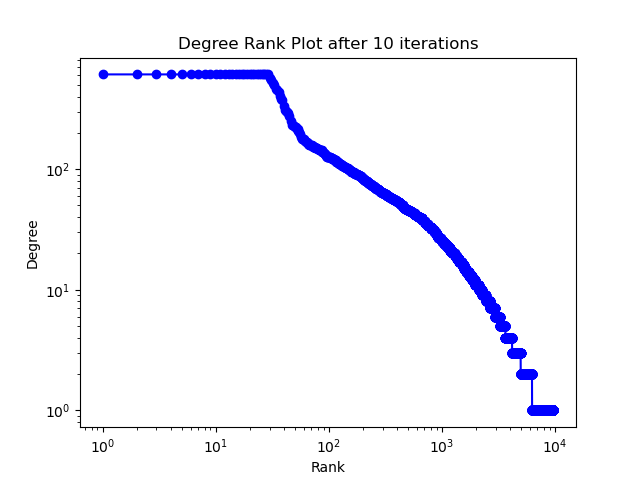
\includegraphics[width=\textwidth]{Prob S movie rank plot - 10 iterations.png}
\end{subfigure}
\hfill
\begin{subfigure}[b]{0.32\textwidth}
    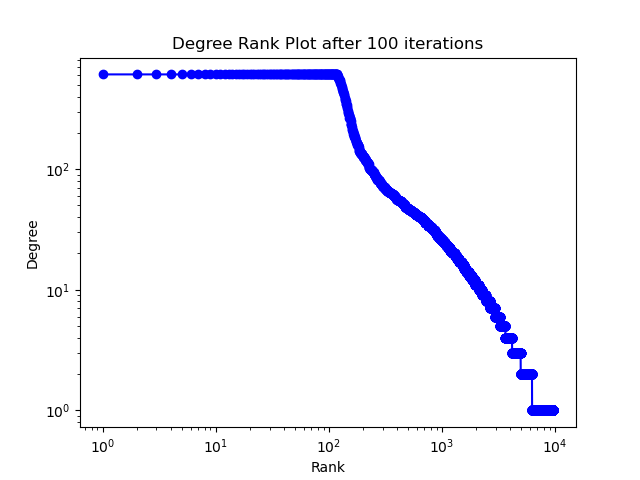
\includegraphics[width=\textwidth]{Prob S movie rank plot - 100 iterations.png}
\end{subfigure}

\vspace{1em} % Add some vertical spacing between the rows

% Second row with three figures
\begin{subfigure}[b]{0.32\textwidth}
    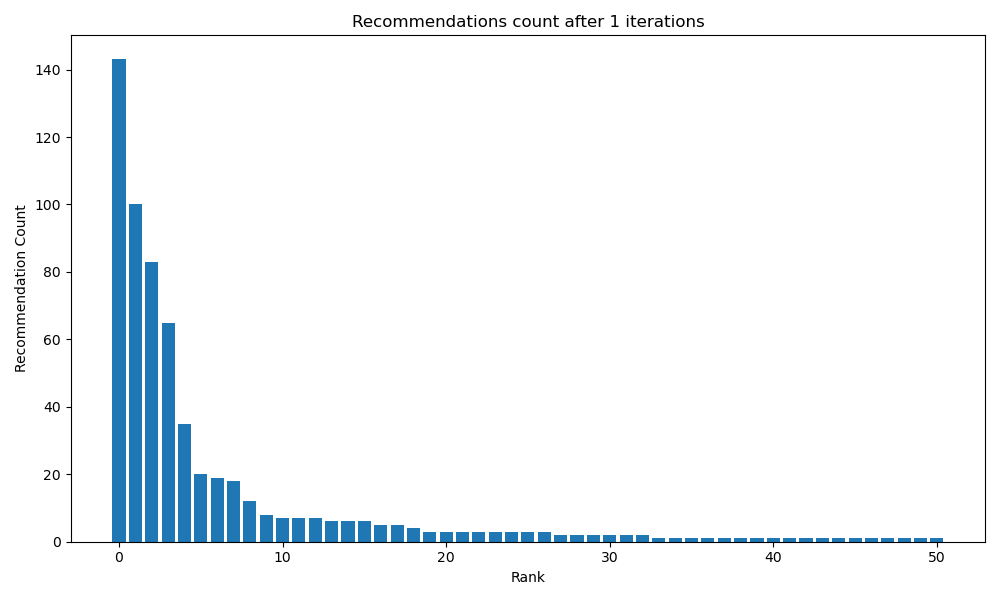
\includegraphics[width=\textwidth]{Prob S movie recommendations - 1 iterations.png}
\end{subfigure}
\hfill
\begin{subfigure}[b]{0.32\textwidth}
    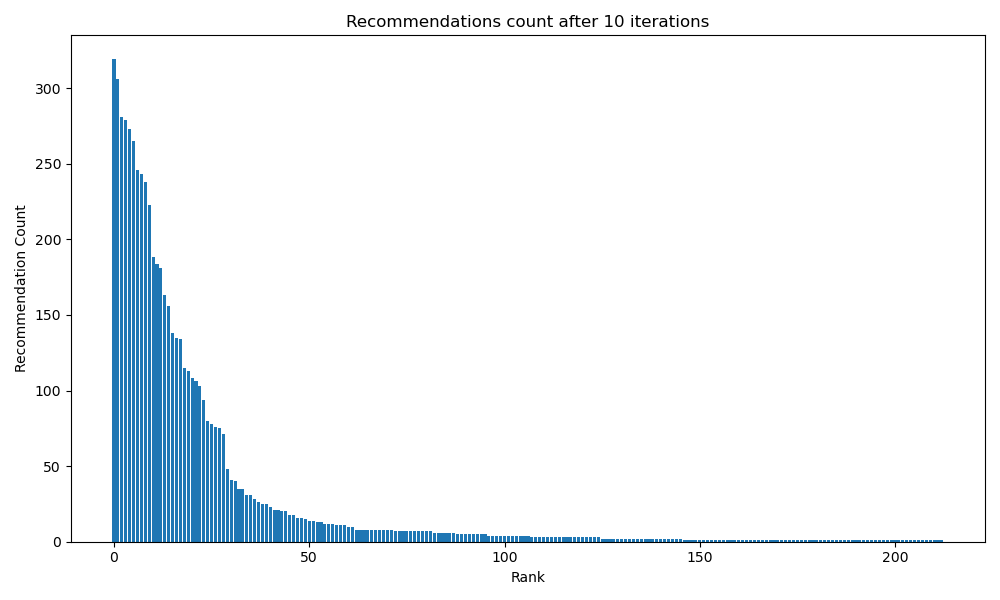
\includegraphics[width=\textwidth]{Prob S movie recommendations - 10 iterations.png}
\end{subfigure}
\hfill
\begin{subfigure}[b]{0.32\textwidth}
    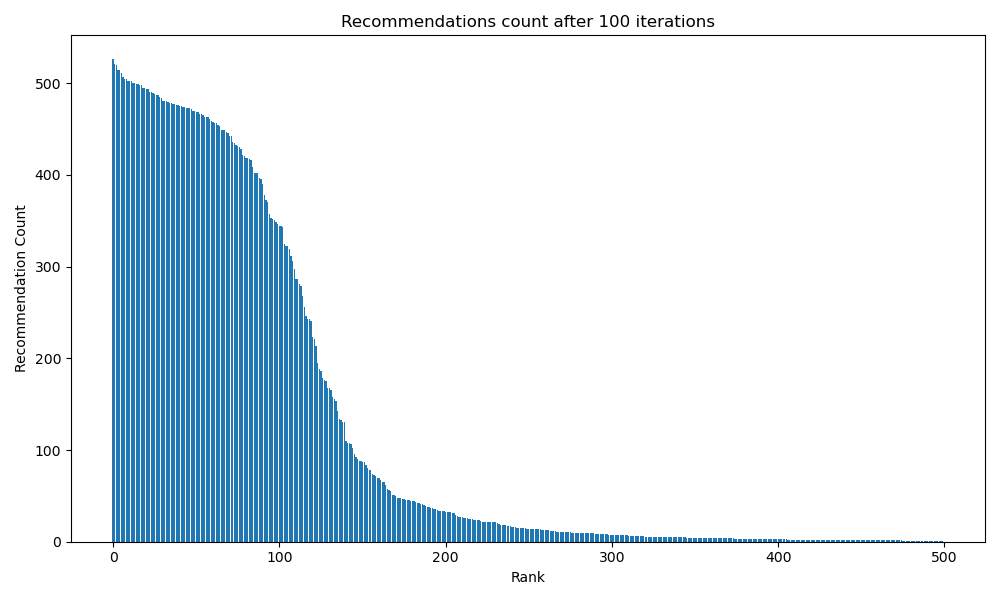
\includegraphics[width=\textwidth]{Prob S movie recommendations - 100 iterations.png}
\end{subfigure}

\caption{ProbS - Recommendation Dynamics}
\label{fig:temporal prob S}

\end{figure}

Figure \ref{fig:temporal heat S} shows the temporal analysis of the binary HeatS algorithm. Unlike ProbS, HeatS distributes its recommendations more evenly among items, as evidenced by the flatter distribution of recommendation counts over iterations. Items less connected in the user-item bipartite network are given relatively higher visibility, shown by the degree of lesser connected movies increasing while that of more connected films stays relatively unchanged. This prevents the dominance of a few movies, giving users recommendations from a broader array of content.

\begin{figure}[!ht]
\centering

% First row with three figures
\begin{subfigure}[b]{0.32\textwidth}
    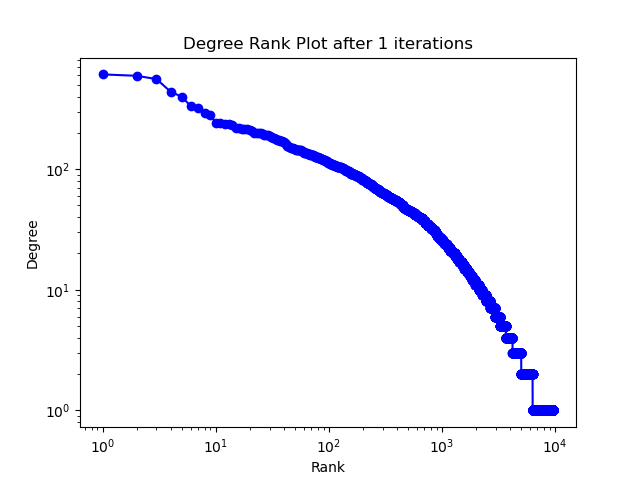
\includegraphics[width=\textwidth]{Heat S movie rank plot - 1 iterations.png}
\end{subfigure}
\hfill
\begin{subfigure}[b]{0.32\textwidth}
    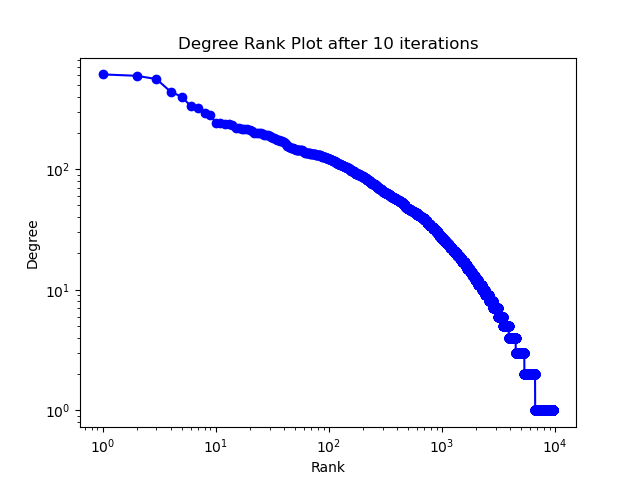
\includegraphics[width=\textwidth]{Heat S movie rank plot - 10 iterations.png}
\end{subfigure}
\hfill
\begin{subfigure}[b]{0.32\textwidth}
    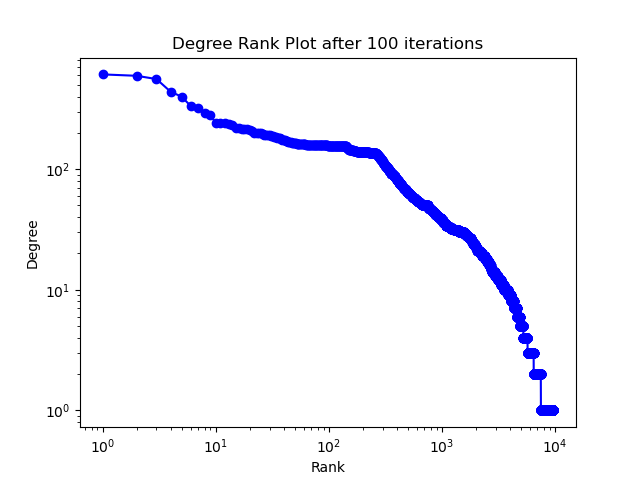
\includegraphics[width=\textwidth]{Heat S movie rank plot - 100 iterations.png}
\end{subfigure}

\vspace{1em} % Add some vertical spacing between the rows

% Second row with three figures
\begin{subfigure}[b]{0.32\textwidth}
    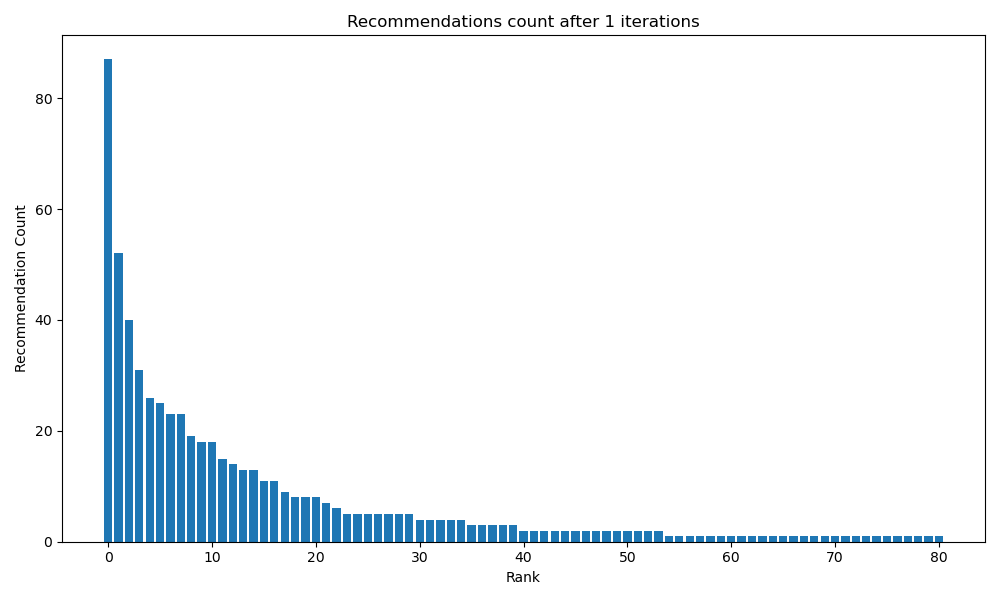
\includegraphics[width=\textwidth]{Heat S movie recommendations - 1 iterations.png}
\end{subfigure}
\hfill
\begin{subfigure}[b]{0.32\textwidth}
    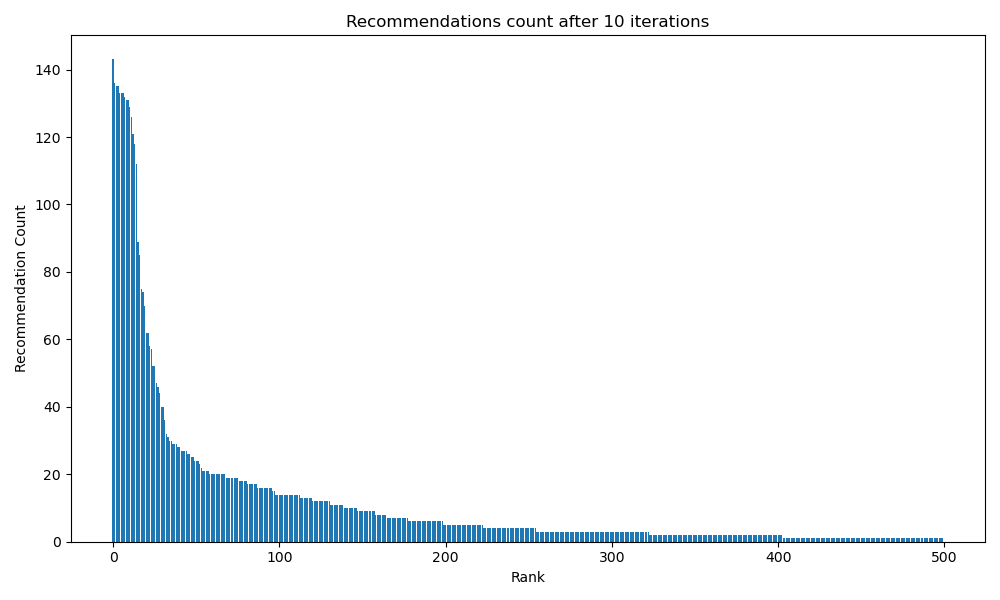
\includegraphics[width=\textwidth]{Heat S movie recommendations - 10 iterations.png}
\end{subfigure}
\hfill
\begin{subfigure}[b]{0.32\textwidth}
    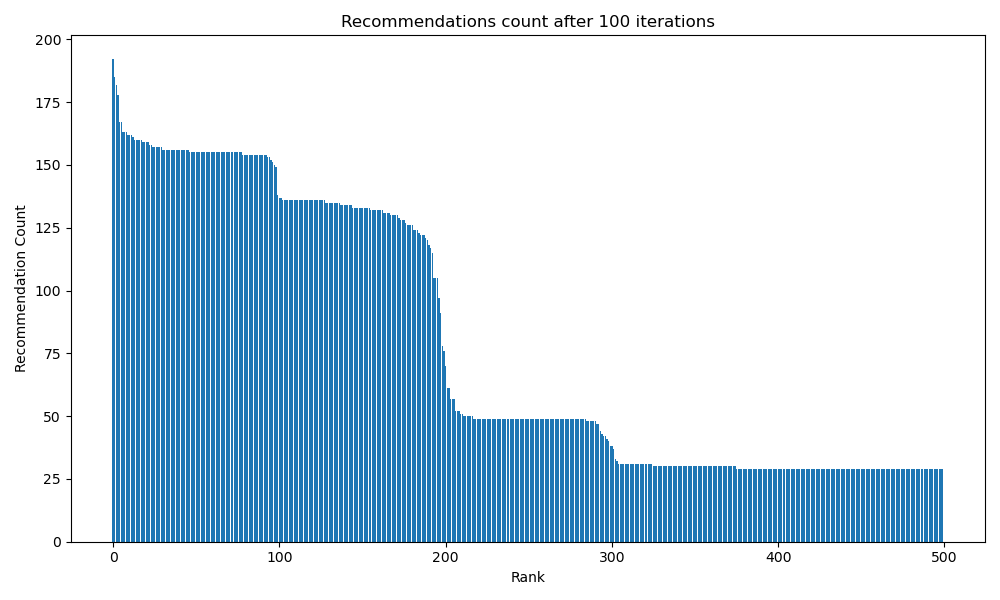
\includegraphics[width=\textwidth]{Heat S movie recommendations - 100 iterations.png}
\end{subfigure}

\caption{HeatS - Recommendation Dynamics}
\label{fig:temporal heat S}

\end{figure}



\subsection{Out of Sample Performance}

In order to evaluate the effectiveness of these recommender system, we perform a train-test split by randomly removing 20\% of each users ratings and subsequently calculate the Area Under the Curve (AUC) and average precision (i.e. percentage of recommendations that were actually liked by the user). The AUC is a performance metric used to evaluate the quality of binary classification models, which seemed a natural way to assess the performance of these algorithms since we can easily normalise the recommendation score given to be between 0 and 1. It represents tradeoff between the true and false positive rates at various threshold settings. The AUC ranges from 0 to 1, where a model with an AUC of 1 perfectly distinguishes between the two classes, and an AUC of 0.5 indicates no discriminative power, equivalent to random guessing. For the evaluation, a movie in the test set is deemed "liked" by a user if its rating exceeds the user's average rating across all movies in the training set, and thus we classify it as a good movie for the algorithm to recommend. To benchmark the results, we also calculate the average precision and AUC for a recommender system simply based on the average rating for each movie.

\begin{figure}[!ht]
    \centering  % Centers the table
    \begin{tabular}{|p{6cm}|r|r|}
        \hline
        \textbf{Model} & \multicolumn{1}{p{4cm}|}{\textbf{AUC}} & \multicolumn{1}{p{4cm}|}{\textbf{Average Precision}}  \\
        \hline
        Using Average Rating & 0.67 & 0.67 \\
        Prob S - uniform weight & 0.57 & 0.62 \\
        Prob S - using ratings & 0.59 & 0.62 \\
        Heat S - uniform weight & 0.51 & 0.54 \\
        Heat S - using ratings & 0.54 & 0.57 \\
        \hline
    \end{tabular}
    \caption{ProbS - Model performance} % Add your caption
    \label{fig:prob s performance} % Label your figure for reference
\end{figure}

As shown in Figure \ref{fig:prob s performance}, both the ProbS and HeatS models perform worse than the recommendations from using a movies average rating, with the incorporations of ratings only resulting in a small improvement. Furthermore, HeatS only performs slightly better than random. This underperformance could be due to data sparsity and the "cold-start problem", where the algorithms struggles to make accurate predictions because of insufficient user-item interaction data. In contrast, average ratings don't rely on user interaction and can recommend popular items effectively.

This said, the poor performance of the random walk models in terms of AUC does not necessarily mean that they are of no use.  One key limitation is that our assessment is based solely on the movies held out in test that a user has already watched. These models might excel at suggesting new and diverse content that aligns with user preferences, yet this aspect remains unmeasured in this setting. This is likely to be particularly true of HeatS, which offers a more diverse array of suggests than ProbS or HeatS, which will often recommend items a user is already aware of.


\section{Collaborative Filtering}

\section{Graphical Neural Networks}

\newpage
\section{Conclusions}
\vspace{1em} 



%\bibliographystyle{plain}
%\bibliography{Bibliography.bib}

\newpage
\printbibliography[heading=bibintoc]

\end{document}